%%%%%%%%%%%%%%%%%%%%%%%%%%%%%%%%%%%%%%%%%%%%%%%%%%%%%%%%%%%%%%%%%%%%
%% I, the copyright holder of this work, release this work into the
%% public domain. This applies worldwide. In some countries this may
%% not be legally possible; if so: I grant anyone the right to use
%% this work for any purpose, without any conditions, unless such
%% conditions are required by law.
%%%%%%%%%%%%%%%%%%%%%%%%%%%%%%%%%%%%%%%%%%%%%%%%%%%%%%%%%%%%%%%%%%%%

\documentclass{beamer}
\usetheme[logopath=./, logo=fig/logo-tu.png]{fibeamer}
\usepackage[utf8]{inputenc}
\usepackage[
  main=english, %% By using `czech` or `slovak` as the main locale
                %% instead of `english`, you can typeset the
                %% presentation in either Czech or Slovak,
                %% respectively.
  czech, slovak %% The additional keys allow foreign texts to be
]{babel}        %% typeset as follows:
%%
%%   \begin{otherlanguage}{czech}   ... \end{otherlanguage}
%%   \begin{otherlanguage}{slovak}  ... \end{otherlanguage}
%%
%% These macros specify information about the presentation
\title{Robust Gate Detection for Autonomous Drone Racing} %% that will be typeset on the
\subtitle{Mid-Term Presentation} %% title page.
\author{Philipp Dürnay\\ \bigskip \bigskip Guido de Croon \hfill	
\includegraphics[width=3cm]{fig/mavlab}\\
	 David M. J. Tax  \hfill 
\includegraphics[width=3cm]{fig/prgroup}%
}
%% These additional packages are used within the document:
\usepackage{ragged2e}  % `\justifying` text
\usepackage{booktabs}  % Tables
\usepackage{tabularx}
\usepackage{tikz}      % Diagrams
\usetikzlibrary{calc, shapes, backgrounds}
\usepackage{amsmath, amssymb}
\usepackage{url}       % `\url`s
\usepackage{listings}  % Code listings
\frenchspacing
\begin{document}
  \frame{\maketitle}

  %\AtBeginSection[2,3,4]{% Print an outline at the beginning of sections
  %  \begin{frame}<beamer>
  %    \frametitle{Outline for Section \thesection}
  %    \tableofcontents[currentsection]
  %  \end{frame}}

  \begin{darkframes}
  	\begin{frame}{Outline}
  		\tableofcontents
  	\end{frame}
	\section{Introduction}
	\subsection{Application}
    \begin{frame}{IROS2018}
    	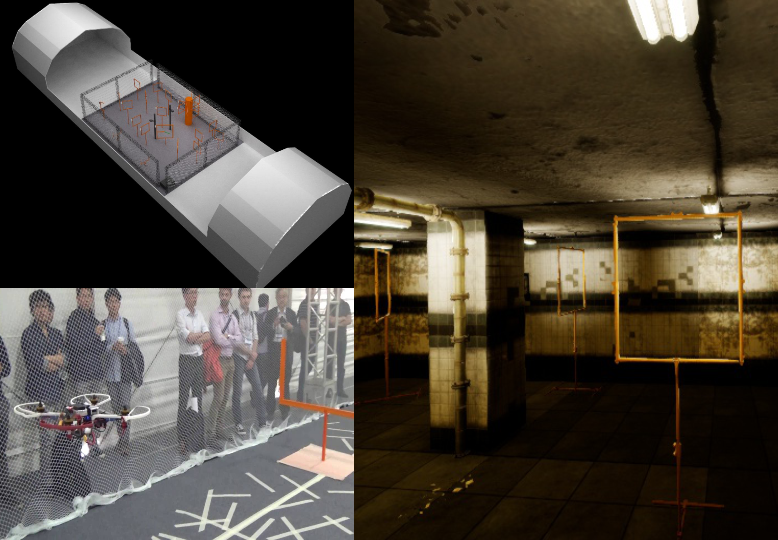
\includegraphics[width=\textwidth]{fig/application}
    \end{frame}
%So we start with the background. The final application will be at the Autonomous Drone Race at the IROS2018 conference in spain. There you have a track that consists of multiple orange gates that need to be passed one after another. So here on the top you see the race court of two years ago. On the bottom you see an example of how a drone looks like. And here on the right you see an example of the training data. So in our method we use these gates to determine our own position. So we detect the gate estimate our own position relative to it and then this goes to the control loop and we fly through. In my thesis I am concerned with the detection of these gates.
    \begin{frame}{Current Method}
       	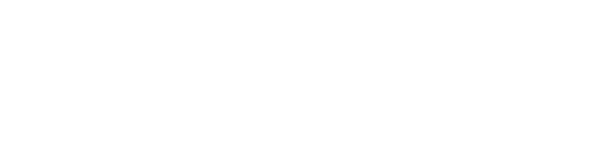
\includegraphics[width=\textwidth]{fig/current_method}
    \end{frame}
%Now currently we have a very basic computer vision method that basically looks for orange pixels and if it finds a square it extracts the corners and together with the known geometry of the gate we can estimate our own position.
%As you can imagine this method is purely colour based and very brittle. You need to tune the colour values depending on the light conditions of the room. And even then if you have strong shadows the method fails. Also it can happend that you are quite far away from the gate and then you don't see the square anymore but only the pole. In this case the method also doesnt work. So we want to improve this by using a learning based approach. As we hope this results in a more robust and flexible method. For example a learning based method you can train if the shapes of the gate change. So this brings me to the underlying research problem. Which can be formulated as follows.
	\subsection{Research Problem}    
	\begin{frame}{Research Problem}
	\textbf{Efficient and robust detection of wire frame objects with limited resources.}
	\end{frame}
 % Since it needs to run on a drone it should be fast and the faster it gets the better for the control, the faster we can fly/ a smaller drone we can use. The wire frame objects we refer to as the objects we want to detect consists only out of a thin frame but I will get back to that later. So I will look at some background in object detection.   
    \section{Background}
    \begin{frame}{Outline for Section \thesection}
    \tableofcontents[currentsection]
	\end{frame}
\subsection{Object Detection}
	\begin{frame}{Object Detection}
	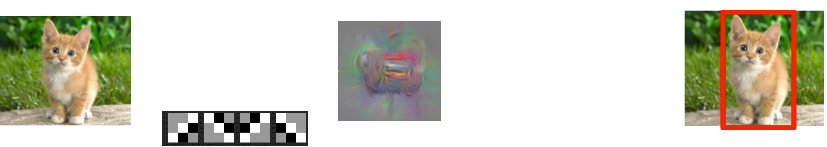
\includegraphics[width=\textwidth]{fig/ObjectDetection}
	\end{frame}
% if you look at object detection on a high level basis, you basically see this pipeline
% You have your input image and at the end you want to have a bounding box that tells you which object is where in the image for example with such a bounding box,
% so usually you preprocess the image by extracting certain features from the image
% so you have filters that look for certain colours or an eye or an ear for example,
% this gives you an internal representation of the image with the important aspects
% then you do two tasks and that is classification and localization so determining the object and the bounding box coordinates
% Now there are different ways for each of these steps but thats it from a high level perspective
% State of the art methods all use convolutional neural networks and the reason that is beliefed to be responsible for that performance is the fact that you can combine all these steps in one model and train it end to end on the task so instead of manually enginnering and training models you combine it all in one.
	\subsection{Convolutional Neural Networks}
		\begin{frame}{Convolutional Networks}
	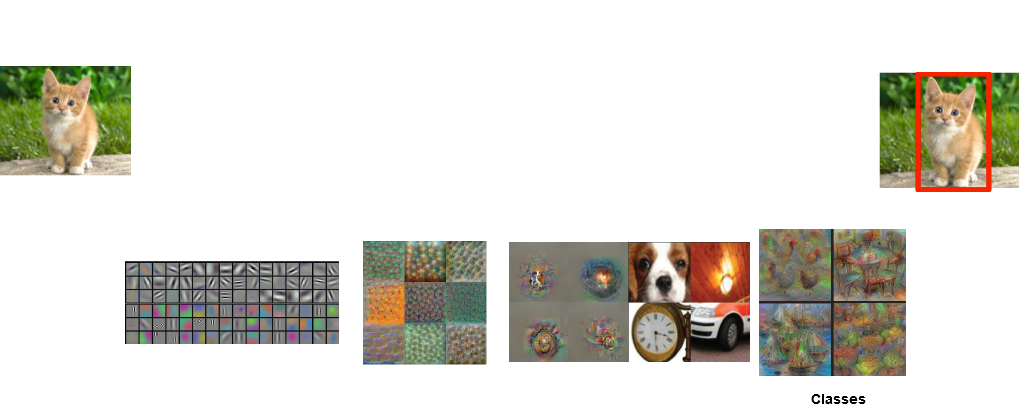
\includegraphics[width=\textwidth]{fig/cnn_mine}
\end{frame}

% So now we can look at an example for a convolutional network and at the different layers. So typically you apply per layer a certain amount of filters, then you apply pooling and non-linearity and you stack several of these filters and at the end you have your output.
% And typically the performance improves the deeper you go. One reason is that the flexibility of the model increases but you can also look at it from another perspective and see what the different layers are responsible for. So when you visualize these filters you usually see how these early layers look for edges, corner and blobs, while higher layers then combine these low level features to more complex parts like eyes, noses and so on.
% Now the draw back of these deep networks is their computational effort, especially the deep one is their huge consumption in energy, computations and memory which makes them not applicable for micro air vehicles.
% But if we now rethink to the objects we want to detect so wire frame objects, racing gates that mostly consist of edges and corners, these final layers should not be very useful. So a much smaller model should actually be sufficient. 
    \section{Approach}
        \begin{frame}{Outline for Section \thesection}
    \tableofcontents[currentsection]
\end{frame}
  \subsection{Method}
    \begin{frame}{Approach}
  Hypothesis: A much smaller network should be able to learn the task.
  \\ \bigskip \bigskip
	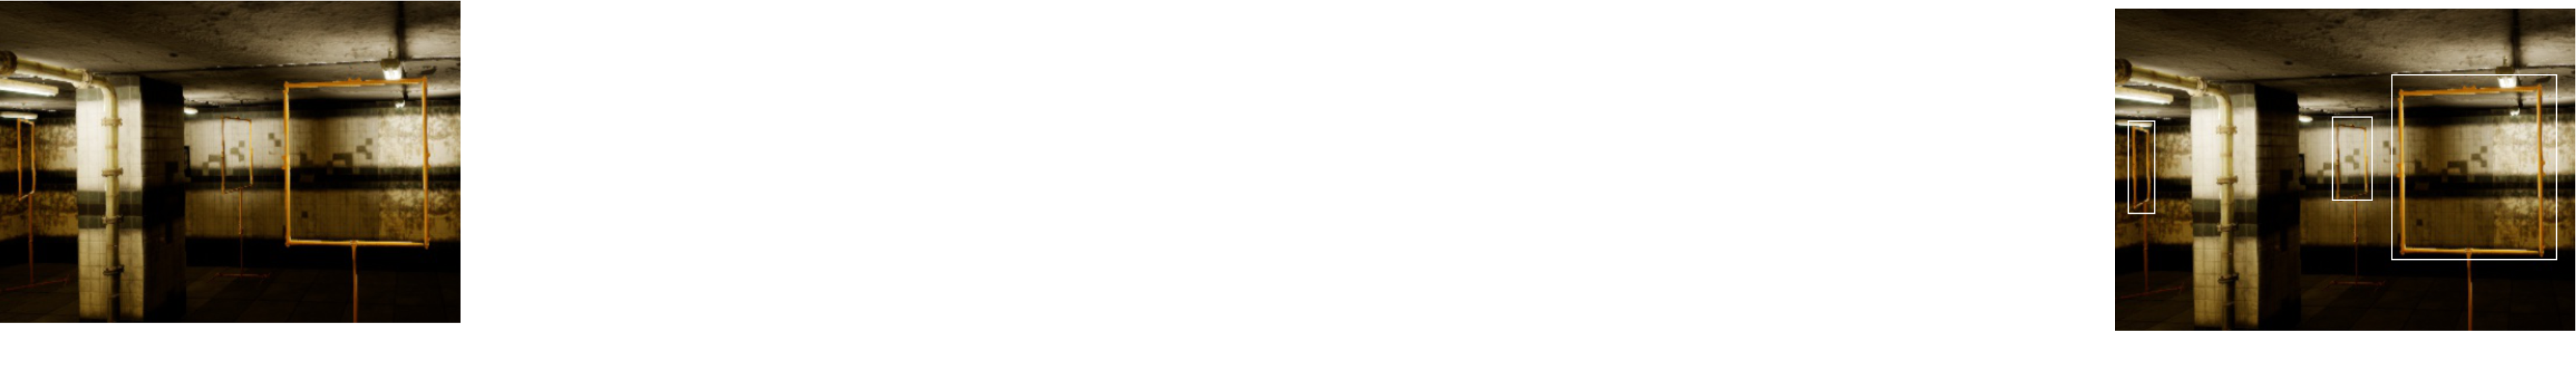
\includegraphics[width=\textwidth]{fig/approach}
    \end{frame}
% Our hypothesis is a much small network should be able to learn the task. So we take a well performing deep object detector and try to scale it down. For now we took the yolo object detector with 23 layers, like you can see here exemplified. And our goal is to make the model smaller and thus also faster. To this end we use an intuitive approach by just modifying the architecture and train the network again.
    
    \subsection{Results}
    \begin{frame}{Results}
    	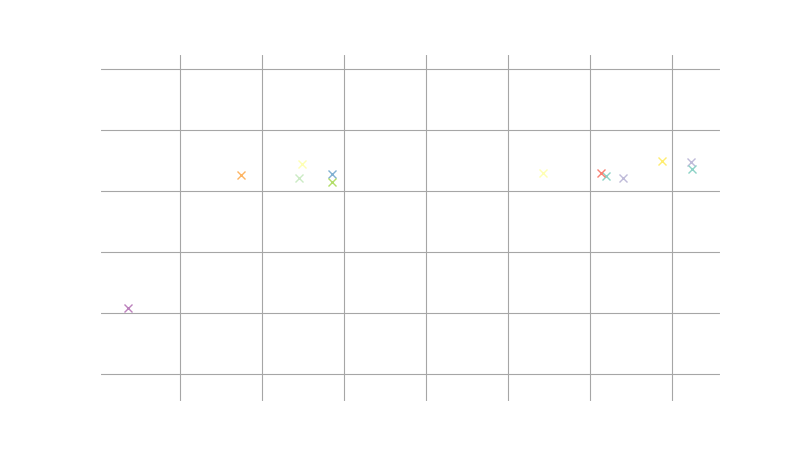
\includegraphics[width=\textwidth]{fig/params_perf}
    \end{frame}
% Here you can see some results we see, mean average precision which is a metric for object detection over the number of weights. We see the original detector as a dot and several of our architectures with different hyperparameters as crosses. And you can see how the performance stays the same although the number of weights is reduced quite a lot. Now of course this is not only because we have a simpler object but also because we only want to detect one class while the original detector detected up to 20 classes.

    \begin{frame}{Results}
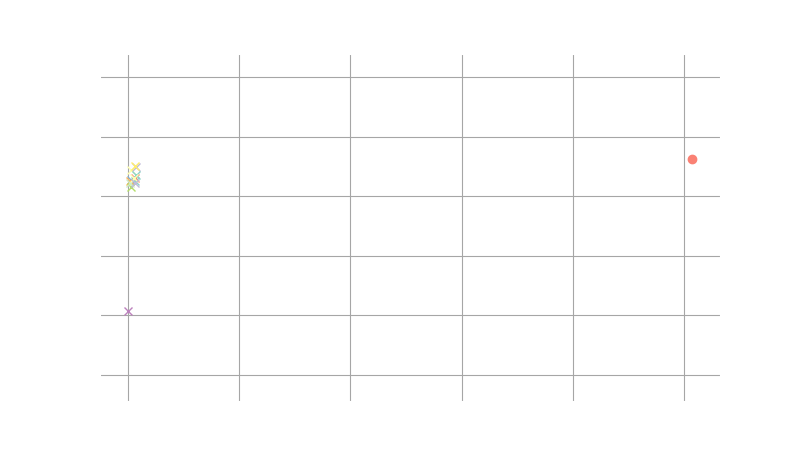
\includegraphics[width=\textwidth]{fig/params_perf_close}
\end{frame}

    \begin{frame}{Results}
	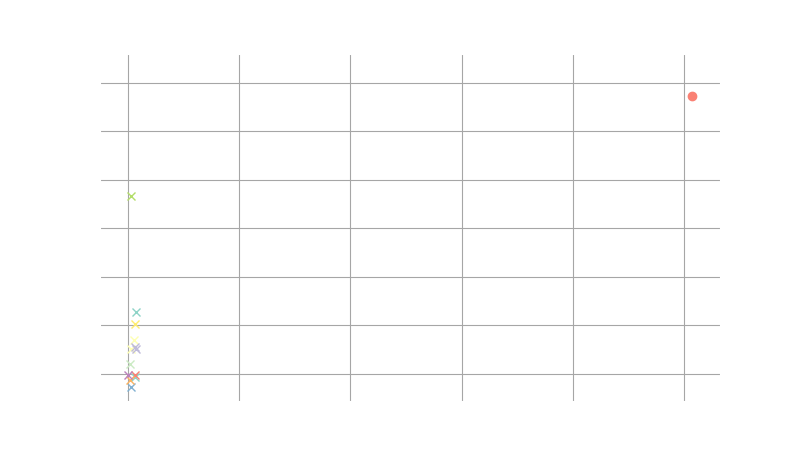
\includegraphics[width=\textwidth]{fig/params_speed}
	\end{frame}

% In the next step we also analyze speed. So these measurements are taken out on the INSY cluster with quite a big GPU. On the drone these values will probably still vary. In total you can see again a huge drop in weights and a boost in performance.

    \begin{frame}{Results}
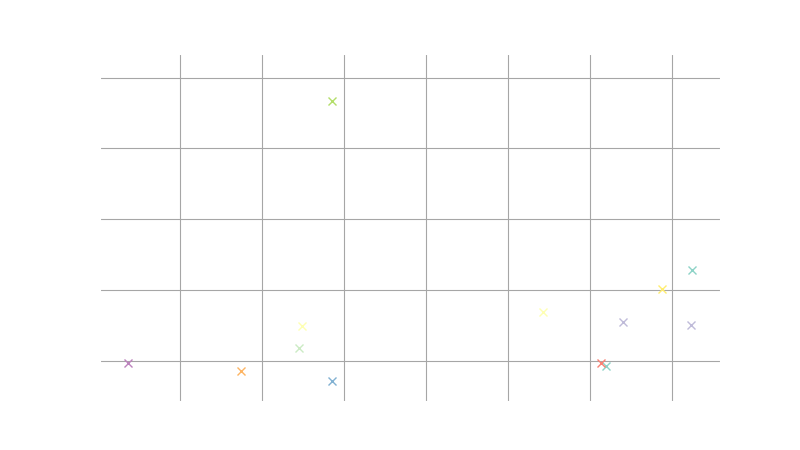
\includegraphics[width=\textwidth]{fig/params_speed_close}
\end{frame}
% However, if we look closer we also see how the boost in speed gets smaller at some point. So reducing the number of weights further does not increase to such a significant speed up anymore. Hence, the bottleneck seems to be somewhere else now.


    \begin{frame}{Results - Examples}
    	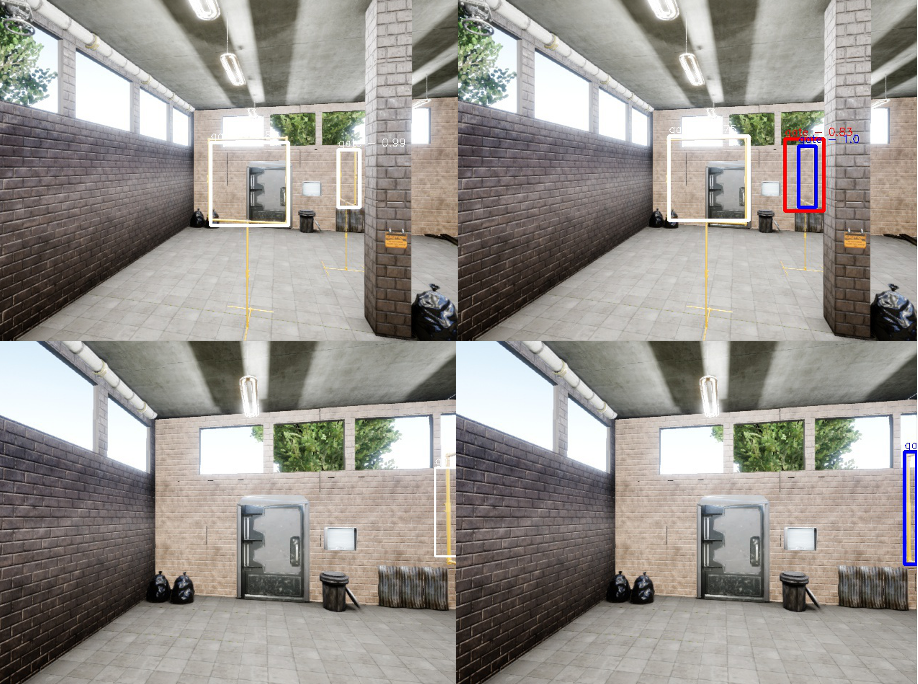
\includegraphics[width=\textwidth]{fig/examples}
	\end{frame}
% Here you see some results, on the left the original yolo model on the right our model with 9 layers. White are correct detections, blue are missed gates and red are false detections. We see how the bigger model produces more accurate bounding boxes and can handle the difficult angles better.

    
    \section{Conclusion}
            \begin{frame}{Outline for Section \thesection}
    \tableofcontents[currentsection]
\end{frame}
    \begin{frame}{Conclusion}

    \begin{itemize}
    	\item Initial assumption confirmed. Much less layers are necessary. However, with less then 9 layers the performance starts dropping.
    	\item Deeper network handles objects in difficult poses better.
    	\item Number of weights is much smaller, however reduction in parameters does not lead equal speed up.
    \end{itemize}
    \end{frame}

    \begin{frame}{Next Steps}
    	\begin{itemize}
    		\item Analysing where most performance/time gets lost
    		\item Investigating further methods to reduce model size/ speed up computations while maintaining accuracy.
    	\end{itemize}
    \end{frame}
    

    \begin{frame}{Questions}
    \centering
\huge ?
    	\end{frame}
    
    
  \end{darkframes}

\end{document}
